%!TEX root = ../main.tex

\section{More Graph Traversals}

We continue talking about graph traversals.

\subsection{Breadth First Search (BFS)}

Let $G = (V, E)$ be a graph and let $s \in V$ be the source. The goal of this
algorithm is to visit all the vertices in the graph. A way to visualize BFS is 
picturing a ripple in the water. At time $t$ the algorithm will visit
nodes a distance $t$ from $s$.

There will three possible states for each vertex. 

\begin{itemize}
    \item Undiscovered: A vertex has not yet been visited.
    \item Discovered: Just visited a vertex but not its neighbors.
    \item Finished: Visited vertex and neighbors.
\end{itemize}

\begin{algorithm}
\caption{Breadth first search}
\begin{algorithmic}
\REQUIRE{$G$ a graph,  $s$ a source vertex}
\STATE{$Q = queue(\{s\})$}
\STATE{$seen = \{ s \}$}
\WHILE{$Q$ is not empty}
\STATE{$v = Q.dequeue()$}
\STATE{visit $v$}
\IF{$v$ not in $seen$}
\STATE{$seen = seen \cup \{v\}$}
\FOR{neighbor $n$ in $v$}
\STATE{$Q = Q \cup \{n\}$}
\ENDFOR
\ENDIF
\ENDWHILE
\end{algorithmic}
\end{algorithm}

We can associate levels with the vertices in BFS. The level of $s$ is
0, the neighbors of $s$ have level 1, and so on. Vertex $v$ is
discovered when we dequeue some vertex $u$, and we will set the level
$l
(v) = l(u) + 1$.

\begin{theorem}
    The level of a vertex $v$ is the smallest number of hops to
get from the source $s$ to $v$.
\end{theorem}

\begin{proof}
    Let $\delta(s, v)$ be the smallest number of hops to get from $s$
    to $v$.
    \begin{itemize}
        \item Claim 1: $\delta(s, v) \leq l(v)$. If $v$ has level $l$,
        then there is a sequence of vertices $s, v_1, ..., v_{l-1}, v$
        with $l(v_1) = 1$, $l(v_2) = 2$, and so on. Each vertex was
        discovered from the previous in the sequence. This constitutes
        a path from $s$ to $v$. The smallest path, $\delta(s, v)$,
        must be therefore smaller or equal to this path.
        \item Claim 2: $\delta(s, v) \geq l(v)$. Suppose for a
        contradiction this claim does not hold. For all the $v$ such
        that
        $\delta(s, v) < l(v)$ find the one with smallest $\delta(s,
        v)$. By definition of $\delta$, there is a path from $s$ to
        $v$ with $\delta(s, v)$ hops. Let $s, ..., u, v$ be the path
        with the fewest hops from $s$ to $v$. What does $u$ look like?
        We know $\delta(s, u) = \delta(s, v) - 1$. By the way we
        constructed
        $v$ as being the smallest that contradicts Claim 2, then $u$
        satisfies Claim 2, so therefore $l(u) \leq
        \delta(s, u) = \delta(s, v) - 1$.
        We also know that $l(v) \leq l(u) + 1$. Putting it all
        together, we have that
        $$
        l(v) \leq l(u) + 1 \leq \delta(s, v)
        $$
        which is a contradiction.
    \end{itemize}
\end{proof}

\begin{remark}
    Look at the edges for which new vertices are discovered. These 
edges form a tree (think of the tree as directed away from $s$).
\end{remark}

\subsection{Depth First Search (DFS)}

The idea is that you explore one path as far as it will go, then
backtrack minimally and repeat. More formally, look at
Algorithm~\ref{alg:dfs}.


\begin{algorithm}
\caption{Depth first search}
\begin{algorithmic}
\REQUIRE{$G$ a graph,  $s$ a source vertex, $seen$ a set}
\STATE{visit $s$}
\STATE{$seen = seen \cup \{ s \}$}
\FOR{each neighbor $n$ of $s$}
\IF{$n$ not in $seen$}
\STATE{recursively call DFS with source $n$}
\ENDIF
\ENDFOR
\end{algorithmic}
\label{alg:dfs}
\end{algorithm}

As in BFS, there will three possible states for each vertex. In BFS
the order of exploration of vertices is the same as the order of
discovery (first in, first out). In DFS, however, we use a stack (or
the recursion stack), so we do last in first out. In other words, the
last discovered vertex is the one first fully explored.

The DFS tree is formed by the set of edges on which new vertices are
discovered.


\begin{lemma}
    If $(u, v)$ is an edge in the graph that is not in the DFS tree,
    then either $u$ is an ancestor of $v$ or $v$ is an ancestor of
    $u$ in the DFS tree.
\end{lemma}

\begin{proof}
    Proof by picture. Do it as an exercise (hint: assume
    contradiction).
\end{proof}


\begin{definition}
The start time $s(u)$ for vertex $u$ is the time for
which DFS of $u$ is invoked, and the finish time $f(u)$ is the time for
which
DFS of $u$ finishes. The duration is the interval from start time to
finish time.
\end{definition}

Note that for all $u, v$ we can't have that $s(u) < s(v) < f(u) <
f(v)$ by the properties of stacks.

Another claim that is useful for DFS is the following. Let's begin
with a wrong, too strong claim.

\begin{lemma}
    (False lemma!). Suppose $u$ is discovered before $v$ and there is a
    path between $u$ and $v$. Then during DFS, $v$ will become a
    descendant of $u$.
\end{lemma}

Why is this wrong? Let's find a counterexample. Consider Figure~\ref{fig:dfs-wrong-lemma}.

\begin{figure}[hpt]
\centering
    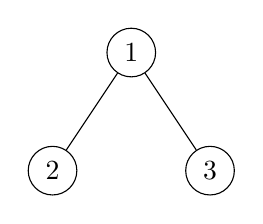
\begin{tikzpicture}[level distance=1.5cm,
                        level 1/.style={sibling distance=2cm}]
  \node[circle, draw=black] {$1$}
    child {node[circle, draw=black] {$2$}} 
    child {node[circle, draw=black] {$3$}};
    \end{tikzpicture}
\caption{Counterexample to the wrong lemma}
\label{fig:dfs-wrong-lemma}
\end{figure}

Suppose DFS visits 2 before 3. There is clearly a path from 2 to 3, 
but 3 is not going to be a descendant of 2. The problem is that the
path between 2 and 3 has vertices that have already been visited.
Let's fix the lemma.

\begin{lemma}
    Suppose $u$ is discovered before $v$ and there is a
    path of undiscovered vertices between $u$ and $v$. Then during
    DFS, $v$ will become a
    descendant of $u$.
\end{lemma}

If you want to prove this, use contradiction.

\section{Connectivity}

\begin{definition}
    A graph is called biconnected if the removal of any vertex leaves
    the graph connected. A graph is called $k$-connected if the
    removal of any $k - 1$ vertices leaves the graph connected.
\end{definition}

A tree is a good example of a connected graph that is not biconnected
(e.g. Figure~\ref{fig:dfs-wrong-lemma}).

\begin{definition}
    A vertex whose removal disconnects the graph is called an
    articulation point.
\end{definition}
 













